\documentclass{report}

%%%%%%%%%%%%%%%%%%%%%%%%%%%%%%%%%
% PACKAGE IMPORTS
%%%%%%%%%%%%%%%%%%%%%%%%%%%%%%%%%


\usepackage[tmargin=2cm,rmargin=1in,lmargin=1in,margin=0.85in,bmargin=2cm,footskip=.2in]{geometry}
\usepackage{amsmath,amsfonts,amsthm,amssymb,mathtools}
\usepackage[varbb]{newpxmath}
\usepackage{xfrac}
\usepackage[makeroom]{cancel}
\usepackage{mathtools}
\usepackage{bookmark}
\usepackage{enumitem}
\usepackage{hyperref,theoremref}
\hypersetup{
	pdftitle={Assignment},
	colorlinks=true, linkcolor=doc!90,
	bookmarksnumbered=true,
	bookmarksopen=true
}
\usepackage[most,many,breakable]{tcolorbox}
\usepackage{xcolor}
\usepackage{varwidth}
\usepackage{varwidth}
\usepackage{etoolbox}
%\usepackage{authblk}
\usepackage{nameref}
\usepackage{multicol,array}
\usepackage{tikz-cd}
\usepackage[ruled,vlined,linesnumbered]{algorithm2e}
\usepackage{comment} % enables the use of multi-line comments (\ifx \fi) 
\usepackage{import}
\usepackage{xifthen}
\usepackage{pdfpages}
\usepackage{transparent}

\newcommand\mycommfont[1]{\footnotesize\ttfamily\textcolor{blue}{#1}}
\SetCommentSty{mycommfont}
\newcommand{\incfig}[1]{%
    \def\svgwidth{\columnwidth}
    \import{./figures/}{#1.pdf_tex}
}

\usepackage{tikzsymbols}
\renewcommand\qedsymbol{$\Laughey$}


%\usepackage{import}
%\usepackage{xifthen}
%\usepackage{pdfpages}
%\usepackage{transparent}


%%%%%%%%%%%%%%%%%%%%%%%%%%%%%%
% SELF MADE COLORS
%%%%%%%%%%%%%%%%%%%%%%%%%%%%%%



\definecolor{myg}{RGB}{56, 140, 70}
\definecolor{myb}{RGB}{45, 111, 177}
\definecolor{myr}{RGB}{199, 68, 64}
\definecolor{mytheorembg}{HTML}{F2F2F9}
\definecolor{mytheoremfr}{HTML}{00007B}
\definecolor{mylenmabg}{HTML}{FFFAF8}
\definecolor{mylenmafr}{HTML}{983b0f}
\definecolor{mypropbg}{HTML}{f2fbfc}
\definecolor{mypropfr}{HTML}{191971}
\definecolor{myexamplebg}{HTML}{F2FBF8}
\definecolor{myexamplefr}{HTML}{88D6D1}
\definecolor{myexampleti}{HTML}{2A7F7F}
\definecolor{mydefinitbg}{HTML}{E5E5FF}
\definecolor{mydefinitfr}{HTML}{3F3FA3}
\definecolor{notesgreen}{RGB}{0,162,0}
\definecolor{myp}{RGB}{197, 92, 212}
\definecolor{mygr}{HTML}{2C3338}
\definecolor{myred}{RGB}{127,0,0}
\definecolor{myyellow}{RGB}{169,121,69}
\definecolor{myexercisebg}{HTML}{F2FBF8}
\definecolor{myexercisefg}{HTML}{88D6D1}


%%%%%%%%%%%%%%%%%%%%%%%%%%%%
% TCOLORBOX SETUPS
%%%%%%%%%%%%%%%%%%%%%%%%%%%%

\setlength{\parindent}{1cm}
%================================
% THEOREM BOX
%================================

\tcbuselibrary{theorems,skins,hooks}
\newtcbtheorem[number within=section]{Theorem}{Theorem}
{%
	enhanced,
	breakable,
	colback = mytheorembg,
	frame hidden,
	boxrule = 0sp,
	borderline west = {2pt}{0pt}{mytheoremfr},
	sharp corners,
	detach title,
	before upper = \tcbtitle\par\smallskip,
	coltitle = mytheoremfr,
	fonttitle = \bfseries\sffamily,
	description font = \mdseries,
	separator sign none,
	segmentation style={solid, mytheoremfr},
}
{th}

\tcbuselibrary{theorems,skins,hooks}
\newtcbtheorem[number within=chapter]{theorem}{Theorem}
{%
	enhanced,
	breakable,
	colback = mytheorembg,
	frame hidden,
	boxrule = 0sp,
	borderline west = {2pt}{0pt}{mytheoremfr},
	sharp corners,
	detach title,
	before upper = \tcbtitle\par\smallskip,
	coltitle = mytheoremfr,
	fonttitle = \bfseries\sffamily,
	description font = \mdseries,
	separator sign none,
	segmentation style={solid, mytheoremfr},
}
{th}


\tcbuselibrary{theorems,skins,hooks}
\newtcolorbox{Theoremcon}
{%
	enhanced
	,breakable
	,colback = mytheorembg
	,frame hidden
	,boxrule = 0sp
	,borderline west = {2pt}{0pt}{mytheoremfr}
	,sharp corners
	,description font = \mdseries
	,separator sign none
}

%================================
% Corollery
%================================
\tcbuselibrary{theorems,skins,hooks}
\newtcbtheorem[number within=section]{Corollary}{Corollary}
{%
	enhanced
	,breakable
	,colback = myp!10
	,frame hidden
	,boxrule = 0sp
	,borderline west = {2pt}{0pt}{myp!85!black}
	,sharp corners
	,detach title
	,before upper = \tcbtitle\par\smallskip
	,coltitle = myp!85!black
	,fonttitle = \bfseries\sffamily
	,description font = \mdseries
	,separator sign none
	,segmentation style={solid, myp!85!black}
}
{th}
\tcbuselibrary{theorems,skins,hooks}
\newtcbtheorem[number within=chapter]{corollary}{Corollary}
{%
	enhanced
	,breakable
	,colback = myp!10
	,frame hidden
	,boxrule = 0sp
	,borderline west = {2pt}{0pt}{myp!85!black}
	,sharp corners
	,detach title
	,before upper = \tcbtitle\par\smallskip
	,coltitle = myp!85!black
	,fonttitle = \bfseries\sffamily
	,description font = \mdseries
	,separator sign none
	,segmentation style={solid, myp!85!black}
}
{th}


%================================
% LENMA
%================================

\tcbuselibrary{theorems,skins,hooks}
\newtcbtheorem[number within=section]{Lenma}{Lenma}
{%
	enhanced,
	breakable,
	colback = mylenmabg,
	frame hidden,
	boxrule = 0sp,
	borderline west = {2pt}{0pt}{mylenmafr},
	sharp corners,
	detach title,
	before upper = \tcbtitle\par\smallskip,
	coltitle = mylenmafr,
	fonttitle = \bfseries\sffamily,
	description font = \mdseries,
	separator sign none,
	segmentation style={solid, mylenmafr},
}
{th}

\tcbuselibrary{theorems,skins,hooks}
\newtcbtheorem[number within=chapter]{lenma}{Lenma}
{%
	enhanced,
	breakable,
	colback = mylenmabg,
	frame hidden,
	boxrule = 0sp,
	borderline west = {2pt}{0pt}{mylenmafr},
	sharp corners,
	detach title,
	before upper = \tcbtitle\par\smallskip,
	coltitle = mylenmafr,
	fonttitle = \bfseries\sffamily,
	description font = \mdseries,
	separator sign none,
	segmentation style={solid, mylenmafr},
}
{th}


%================================
% PROPOSITION
%================================

\tcbuselibrary{theorems,skins,hooks}
\newtcbtheorem[number within=section]{Prop}{Proposition}
{%
	enhanced,
	breakable,
	colback = mypropbg,
	frame hidden,
	boxrule = 0sp,
	borderline west = {2pt}{0pt}{mypropfr},
	sharp corners,
	detach title,
	before upper = \tcbtitle\par\smallskip,
	coltitle = mypropfr,
	fonttitle = \bfseries\sffamily,
	description font = \mdseries,
	separator sign none,
	segmentation style={solid, mypropfr},
}
{th}

\tcbuselibrary{theorems,skins,hooks}
\newtcbtheorem[number within=chapter]{prop}{Proposition}
{%
	enhanced,
	breakable,
	colback = mypropbg,
	frame hidden,
	boxrule = 0sp,
	borderline west = {2pt}{0pt}{mypropfr},
	sharp corners,
	detach title,
	before upper = \tcbtitle\par\smallskip,
	coltitle = mypropfr,
	fonttitle = \bfseries\sffamily,
	description font = \mdseries,
	separator sign none,
	segmentation style={solid, mypropfr},
}
{th}


%================================
% CLAIM
%================================

\tcbuselibrary{theorems,skins,hooks}
\newtcbtheorem[number within=section]{claim}{Claim}
{%
	enhanced
	,breakable
	,colback = myg!10
	,frame hidden
	,boxrule = 0sp
	,borderline west = {2pt}{0pt}{myg}
	,sharp corners
	,detach title
	,before upper = \tcbtitle\par\smallskip
	,coltitle = myg!85!black
	,fonttitle = \bfseries\sffamily
	,description font = \mdseries
	,separator sign none
	,segmentation style={solid, myg!85!black}
}
{th}



%================================
% Exercise
%================================

\tcbuselibrary{theorems,skins,hooks}
\newtcbtheorem[number within=section]{Exercise}{Exercise}
{%
	enhanced,
	breakable,
	colback = myexercisebg,
	frame hidden,
	boxrule = 0sp,
	borderline west = {2pt}{0pt}{myexercisefg},
	sharp corners,
	detach title,
	before upper = \tcbtitle\par\smallskip,
	coltitle = myexercisefg,
	fonttitle = \bfseries\sffamily,
	description font = \mdseries,
	separator sign none,
	segmentation style={solid, myexercisefg},
}
{th}

\tcbuselibrary{theorems,skins,hooks}
\newtcbtheorem[number within=chapter]{exercise}{Exercise}
{%
	enhanced,
	breakable,
	colback = myexercisebg,
	frame hidden,
	boxrule = 0sp,
	borderline west = {2pt}{0pt}{myexercisefg},
	sharp corners,
	detach title,
	before upper = \tcbtitle\par\smallskip,
	coltitle = myexercisefg,
	fonttitle = \bfseries\sffamily,
	description font = \mdseries,
	separator sign none,
	segmentation style={solid, myexercisefg},
}
{th}

%================================
% EXAMPLE BOX
%================================

\newtcbtheorem[number within=section]{Example}{Example}
{%
	colback = myexamplebg
	,breakable
	,colframe = myexamplefr
	,coltitle = myexampleti
	,boxrule = 1pt
	,sharp corners
	,detach title
	,before upper=\tcbtitle\par\smallskip
	,fonttitle = \bfseries
	,description font = \mdseries
	,separator sign none
	,description delimiters parenthesis
}
{ex}

\newtcbtheorem[number within=chapter]{example}{Example}
{%
	colback = myexamplebg
	,breakable
	,colframe = myexamplefr
	,coltitle = myexampleti
	,boxrule = 1pt
	,sharp corners
	,detach title
	,before upper=\tcbtitle\par\smallskip
	,fonttitle = \bfseries
	,description font = \mdseries
	,separator sign none
	,description delimiters parenthesis
}
{ex}

%================================
% DEFINITION BOX
%================================

\newtcbtheorem[number within=section]{Definition}{Definition}{enhanced,
	before skip=2mm,after skip=2mm, colback=red!5,colframe=red!80!black,boxrule=0.5mm,
	attach boxed title to top left={xshift=1cm,yshift*=1mm-\tcboxedtitleheight}, varwidth boxed title*=-3cm,
	boxed title style={frame code={
					\path[fill=tcbcolback]
					([yshift=-1mm,xshift=-1mm]frame.north west)
					arc[start angle=0,end angle=180,radius=1mm]
					([yshift=-1mm,xshift=1mm]frame.north east)
					arc[start angle=180,end angle=0,radius=1mm];
					\path[left color=tcbcolback!60!black,right color=tcbcolback!60!black,
						middle color=tcbcolback!80!black]
					([xshift=-2mm]frame.north west) -- ([xshift=2mm]frame.north east)
					[rounded corners=1mm]-- ([xshift=1mm,yshift=-1mm]frame.north east)
					-- (frame.south east) -- (frame.south west)
					-- ([xshift=-1mm,yshift=-1mm]frame.north west)
					[sharp corners]-- cycle;
				},interior engine=empty,
		},
	fonttitle=\bfseries,
	title={#2},#1}{def}
\newtcbtheorem[number within=chapter]{definition}{Definition}{enhanced,
	before skip=2mm,after skip=2mm, colback=red!5,colframe=red!80!black,boxrule=0.5mm,
	attach boxed title to top left={xshift=1cm,yshift*=1mm-\tcboxedtitleheight}, varwidth boxed title*=-3cm,
	boxed title style={frame code={
					\path[fill=tcbcolback]
					([yshift=-1mm,xshift=-1mm]frame.north west)
					arc[start angle=0,end angle=180,radius=1mm]
					([yshift=-1mm,xshift=1mm]frame.north east)
					arc[start angle=180,end angle=0,radius=1mm];
					\path[left color=tcbcolback!60!black,right color=tcbcolback!60!black,
						middle color=tcbcolback!80!black]
					([xshift=-2mm]frame.north west) -- ([xshift=2mm]frame.north east)
					[rounded corners=1mm]-- ([xshift=1mm,yshift=-1mm]frame.north east)
					-- (frame.south east) -- (frame.south west)
					-- ([xshift=-1mm,yshift=-1mm]frame.north west)
					[sharp corners]-- cycle;
				},interior engine=empty,
		},
	fonttitle=\bfseries,
	title={#2},#1}{def}



%================================
% Solution BOX
%================================

\makeatletter
\newtcbtheorem{question}{Question}{enhanced,
	breakable,
	colback=white,
	colframe=myb!80!black,
	attach boxed title to top left={yshift*=-\tcboxedtitleheight},
	fonttitle=\bfseries,
	title={#2},
	boxed title size=title,
	boxed title style={%
			sharp corners,
			rounded corners=northwest,
			colback=tcbcolframe,
			boxrule=0pt,
		},
	underlay boxed title={%
			\path[fill=tcbcolframe] (title.south west)--(title.south east)
			to[out=0, in=180] ([xshift=5mm]title.east)--
			(title.center-|frame.east)
			[rounded corners=\kvtcb@arc] |-
			(frame.north) -| cycle;
		},
	#1
}{def}
\makeatother

%================================
% SOLUTION BOX
%================================

\makeatletter
\newtcolorbox{solution}{enhanced,
	breakable,
	colback=white,
	colframe=myg!80!black,
	attach boxed title to top left={yshift*=-\tcboxedtitleheight},
	title=Solution,
	boxed title size=title,
	boxed title style={%
			sharp corners,
			rounded corners=northwest,
			colback=tcbcolframe,
			boxrule=0pt,
		},
	underlay boxed title={%
			\path[fill=tcbcolframe] (title.south west)--(title.south east)
			to[out=0, in=180] ([xshift=5mm]title.east)--
			(title.center-|frame.east)
			[rounded corners=\kvtcb@arc] |-
			(frame.north) -| cycle;
		},
}
\makeatother

%================================
% Question BOX
%================================

\makeatletter
\newtcbtheorem{qstion}{Question}{enhanced,
	breakable,
	colback=white,
	colframe=mygr,
	attach boxed title to top left={yshift*=-\tcboxedtitleheight},
	fonttitle=\bfseries,
	title={#2},
	boxed title size=title,
	boxed title style={%
			sharp corners,
			rounded corners=northwest,
			colback=tcbcolframe,
			boxrule=0pt,
		},
	underlay boxed title={%
			\path[fill=tcbcolframe] (title.south west)--(title.south east)
			to[out=0, in=180] ([xshift=5mm]title.east)--
			(title.center-|frame.east)
			[rounded corners=\kvtcb@arc] |-
			(frame.north) -| cycle;
		},
	#1
}{def}
\makeatother

\newtcbtheorem[number within=chapter]{wconc}{Wrong Concept}{
	breakable,
	enhanced,
	colback=white,
	colframe=myr,
	arc=0pt,
	outer arc=0pt,
	fonttitle=\bfseries\sffamily\large,
	colbacktitle=myr,
	attach boxed title to top left={},
	boxed title style={
			enhanced,
			skin=enhancedfirst jigsaw,
			arc=3pt,
			bottom=0pt,
			interior style={fill=myr}
		},
	#1
}{def}



%================================
% NOTE BOX
%================================

\usetikzlibrary{arrows,calc,shadows.blur}
\tcbuselibrary{skins}
\newtcolorbox{note}[1][]{%
	enhanced jigsaw,
	colback=gray!20!white,%
	colframe=gray!80!black,
	size=small,
	boxrule=1pt,
	title=\textbf{Note:-},
	halign title=flush center,
	coltitle=black,
	breakable,
	drop shadow=black!50!white,
	attach boxed title to top left={xshift=1cm,yshift=-\tcboxedtitleheight/2,yshifttext=-\tcboxedtitleheight/2},
	minipage boxed title=1.5cm,
	boxed title style={%
			colback=white,
			size=fbox,
			boxrule=1pt,
			boxsep=2pt,
			underlay={%
					\coordinate (dotA) at ($(interior.west) + (-0.5pt,0)$);
					\coordinate (dotB) at ($(interior.east) + (0.5pt,0)$);
					\begin{scope}
						\clip (interior.north west) rectangle ([xshift=3ex]interior.east);
						\filldraw [white, blur shadow={shadow opacity=60, shadow yshift=-.75ex}, rounded corners=2pt] (interior.north west) rectangle (interior.south east);
					\end{scope}
					\begin{scope}[gray!80!black]
						\fill (dotA) circle (2pt);
						\fill (dotB) circle (2pt);
					\end{scope}
				},
		},
	#1,
}

%%%%%%%%%%%%%%%%%%%%%%%%%%%%%%
% SELF MADE COMMANDS
%%%%%%%%%%%%%%%%%%%%%%%%%%%%%%


\newcommand{\thm}[2]{\begin{Theorem}{#1}{}#2\end{Theorem}}
\newcommand{\cor}[2]{\begin{Corollary}{#1}{}#2\end{Corollary}}
\newcommand{\mlenma}[2]{\begin{Lenma}{#1}{}#2\end{Lenma}}
\newcommand{\mprop}[2]{\begin{Prop}{#1}{}#2\end{Prop}}
\newcommand{\clm}[3]{\begin{claim}{#1}{#2}#3\end{claim}}
\newcommand{\wc}[2]{\begin{wconc}{#1}{}\setlength{\parindent}{1cm}#2\end{wconc}}
\newcommand{\thmcon}[1]{\begin{Theoremcon}{#1}\end{Theoremcon}}
\newcommand{\ex}[2]{\begin{Example}{#1}{}#2\end{Example}}
\newcommand{\dfn}[2]{\begin{Definition}[colbacktitle=red!75!black]{#1}{}#2\end{Definition}}
\newcommand{\dfnc}[2]{\begin{definition}[colbacktitle=red!75!black]{#1}{}#2\end{definition}}
\newcommand{\qs}[2]{\begin{question}{#1}{}#2\end{question}}
\newcommand{\pf}[2]{\begin{myproof}[#1]#2\end{myproof}}
\newcommand{\nt}[1]{\begin{note}#1\end{note}}

\newcommand*\circled[1]{\tikz[baseline=(char.base)]{
		\node[shape=circle,draw,inner sep=1pt] (char) {#1};}}
\newcommand\getcurrentref[1]{%
	\ifnumequal{\value{#1}}{0}
	{??}
	{\the\value{#1}}%
}
\newcommand{\getCurrentSectionNumber}{\getcurrentref{section}}
\newenvironment{myproof}[1][\proofname]{%
	\proof[\bfseries #1: ]%
}{\endproof}

\newcommand{\mclm}[2]{\begin{myclaim}[#1]#2\end{myclaim}}
\newenvironment{myclaim}[1][\claimname]{\proof[\bfseries #1: ]}{}

\newcounter{mylabelcounter}

\makeatletter
\newcommand{\setword}[2]{%
	\phantomsection
	#1\def\@currentlabel{\unexpanded{#1}}\label{#2}%
}
\makeatother




\tikzset{
	symbol/.style={
			draw=none,
			every to/.append style={
					edge node={node [sloped, allow upside down, auto=false]{$#1$}}}
		}
}


% deliminators
\DeclarePairedDelimiter{\abs}{\lvert}{\rvert}
\DeclarePairedDelimiter{\norm}{\lVert}{\rVert}

\DeclarePairedDelimiter{\ceil}{\lceil}{\rceil}
\DeclarePairedDelimiter{\floor}{\lfloor}{\rfloor}
\DeclarePairedDelimiter{\round}{\lfloor}{\rceil}

\newsavebox\diffdbox
\newcommand{\slantedromand}{{\mathpalette\makesl{d}}}
\newcommand{\makesl}[2]{%
\begingroup
\sbox{\diffdbox}{$\mathsurround=0pt#1\mathrm{#2}$}%
\pdfsave
\pdfsetmatrix{1 0 0.2 1}%
\rlap{\usebox{\diffdbox}}%
\pdfrestore
\hskip\wd\diffdbox
\endgroup
}
\newcommand{\dd}[1][]{\ensuremath{\mathop{}\!\ifstrempty{#1}{%
\slantedromand\@ifnextchar^{\hspace{0.2ex}}{\hspace{0.1ex}}}%
{\slantedromand\hspace{0.2ex}^{#1}}}}
\ProvideDocumentCommand\dv{o m g}{%
  \ensuremath{%
    \IfValueTF{#3}{%
      \IfNoValueTF{#1}{%
        \frac{\dd #2}{\dd #3}%
      }{%
        \frac{\dd^{#1} #2}{\dd #3^{#1}}%
      }%
    }{%
      \IfNoValueTF{#1}{%
        \frac{\dd}{\dd #2}%
      }{%
        \frac{\dd^{#1}}{\dd #2^{#1}}%
      }%
    }%
  }%
}
\providecommand*{\pdv}[3][]{\frac{\partial^{#1}#2}{\partial#3^{#1}}}
%  - others
\DeclareMathOperator{\Lap}{\mathcal{L}}
\DeclareMathOperator{\Var}{Var} % varience
\DeclareMathOperator{\Cov}{Cov} % covarience
\DeclareMathOperator{\E}{E} % expected

% Since the amsthm package isn't loaded

% I prefer the slanted \leq
\let\oldleq\leq % save them in case they're every wanted
\let\oldgeq\geq
\renewcommand{\leq}{\leqslant}
\renewcommand{\geq}{\geqslant}

% % redefine matrix env to allow for alignment, use r as default
% \renewcommand*\env@matrix[1][r]{\hskip -\arraycolsep
%     \let\@ifnextchar\new@ifnextchar
%     \array{*\c@MaxMatrixCols #1}}


%\usepackage{framed}
%\usepackage{titletoc}
%\usepackage{etoolbox}
%\usepackage{lmodern}


%\patchcmd{\tableofcontents}{\contentsname}{\sffamily\contentsname}{}{}

%\renewenvironment{leftbar}
%{\def\FrameCommand{\hspace{6em}%
%		{\color{myyellow}\vrule width 2pt depth 6pt}\hspace{1em}}%
%	\MakeFramed{\parshape 1 0cm \dimexpr\textwidth-6em\relax\FrameRestore}\vskip2pt%
%}
%{\endMakeFramed}

%\titlecontents{chapter}
%[0em]{\vspace*{2\baselineskip}}
%{\parbox{4.5em}{%
%		\hfill\Huge\sffamily\bfseries\color{myred}\thecontentspage}%
%	\vspace*{-2.3\baselineskip}\leftbar\textsc{\small\chaptername~\thecontentslabel}\\\sffamily}
%{}{\endleftbar}
%\titlecontents{section}
%[8.4em]
%{\sffamily\contentslabel{3em}}{}{}
%{\hspace{0.5em}\nobreak\itshape\color{myred}\contentspage}
%\titlecontents{subsection}
%[8.4em]
%{\sffamily\contentslabel{3em}}{}{}  
%{\hspace{0.5em}\nobreak\itshape\color{myred}\contentspage}



%%%%%%%%%%%%%%%%%%%%%%%%%%%%%%%%%%%%%%%%%%%
% TABLE OF CONTENTS
%%%%%%%%%%%%%%%%%%%%%%%%%%%%%%%%%%%%%%%%%%%

\usepackage{tikz}
\definecolor{doc}{RGB}{0,60,110}
\usepackage{titletoc}
\contentsmargin{0cm}
\titlecontents{chapter}[3.7pc]
{\addvspace{30pt}%
	\begin{tikzpicture}[remember picture, overlay]%
		\draw[fill=doc!60,draw=doc!60] (-7,-.1) rectangle (-0.9,.5);%
		\pgftext[left,x=-3.5cm,y=0.2cm]{\color{white}\Large\sc\bfseries Chapter\ \thecontentslabel};%
	\end{tikzpicture}\color{doc!60}\large\sc\bfseries}%
{}
{}
{\;\titlerule\;\large\sc\bfseries Page \thecontentspage
	\begin{tikzpicture}[remember picture, overlay]
		\draw[fill=doc!60,draw=doc!60] (2pt,0) rectangle (4,0.1pt);
	\end{tikzpicture}}%
\titlecontents{section}[3.7pc]
{\addvspace{2pt}}
{\contentslabel[\thecontentslabel]{2pc}}
{}
{\hfill\small \thecontentspage}
[]

\titlecontents*{subsection}[4.7pc] % Mayor indentación para subsecciones
{\addvspace{1pt}\small} % Espaciado más limpio
{\thecontentslabel\quad} % Mostrar número de subsección (1.1.1, 1.1.2)
{}
{\hfill\small\thecontentspage\\} % Alinear el número de página correctamente


\makeatletter
\renewcommand{\tableofcontents}{%
	\chapter*{%
	  \vspace*{-20\p@}%
	  \begin{tikzpicture}[remember picture, overlay]%
		  \pgftext[right,x=15cm,y=0.2cm]{\color{doc!60}\Huge\sc\bfseries \contentsname};%
		  \draw[fill=doc!60,draw=doc!60] (13,-.75) rectangle (20,1);%
		  \clip (13,-.75) rectangle (20,1);
		  \pgftext[right,x=15cm,y=0.2cm]{\color{white}\Huge\sc\bfseries \contentsname};%
	  \end{tikzpicture}}%
	\@starttoc{toc}}
\makeatother

 % revisar en preamble \setcounter{tocdepth}{3}
%From M275 "Topology" at SJSU
\newcommand{\id}{\mathrm{id}}
\newcommand{\taking}[1]{\xrightarrow{#1}}
\newcommand{\inv}{^{-1}}

%From M170 "Introduction to Graph Theory" at SJSU
\DeclareMathOperator{\diam}{diam}
\DeclareMathOperator{\ord}{ord}
\newcommand{\defeq}{\overset{\mathrm{def}}{=}}

%From the USAMO .tex files
\newcommand{\ts}{\textsuperscript}
\newcommand{\dg}{^\circ}
\newcommand{\ii}{\item}

% % From Math 55 and Math 145 at Harvard
% \newenvironment{subproof}[1][Proof]{%
% \begin{proof}[#1] \renewcommand{\qedsymbol}{$\blacksquare$}}%
% {\end{proof}}

\newcommand{\liff}{\leftrightarrow}
\newcommand{\lthen}{\rightarrow}
\newcommand{\opname}{\operatorname}
\newcommand{\surjto}{\twoheadrightarrow}
\newcommand{\injto}{\hookrightarrow}
\newcommand{\On}{\mathrm{On}} % ordinals
\DeclareMathOperator{\img}{im} % Image
\DeclareMathOperator{\Img}{Im} % Image
\DeclareMathOperator{\coker}{coker} % Cokernel
\DeclareMathOperator{\Coker}{Coker} % Cokernel
\DeclareMathOperator{\Ker}{Ker} % Kernel
\DeclareMathOperator{\rank}{rank}
\DeclareMathOperator{\Spec}{Spec} % spectrum
\DeclareMathOperator{\Tr}{Tr} % trace
\DeclareMathOperator{\pr}{pr} % projection
\DeclareMathOperator{\ext}{ext} % extension
\DeclareMathOperator{\pred}{pred} % predecessor
\DeclareMathOperator{\dom}{dom} % domain
\DeclareMathOperator{\ran}{ran} % range
\DeclareMathOperator{\Hom}{Hom} % homomorphism
\DeclareMathOperator{\Mor}{Mor} % morphisms
\DeclareMathOperator{\End}{End} % endomorphism

\newcommand{\eps}{\epsilon}
\newcommand{\veps}{\varepsilon}
\newcommand{\ol}{\overline}
\newcommand{\ul}{\underline}
\newcommand{\wt}{\widetilde}
\newcommand{\wh}{\widehat}
\newcommand{\vocab}[1]{\textbf{\color{blue} #1}}
\providecommand{\half}{\frac{1}{2}}
\newcommand{\dang}{\measuredangle} %% Directed angle
\newcommand{\ray}[1]{\overrightarrow{#1}}
\newcommand{\seg}[1]{\overline{#1}}
\newcommand{\arc}[1]{\wideparen{#1}}
\DeclareMathOperator{\cis}{cis}
\DeclareMathOperator*{\lcm}{lcm}
\DeclareMathOperator*{\argmin}{arg min}
\DeclareMathOperator*{\argmax}{arg max}
\newcommand{\cycsum}{\sum_{\mathrm{cyc}}}
\newcommand{\symsum}{\sum_{\mathrm{sym}}}
\newcommand{\cycprod}{\prod_{\mathrm{cyc}}}
\newcommand{\symprod}{\prod_{\mathrm{sym}}}
\newcommand{\Qed}{\begin{flushright}\qed\end{flushright}}
\newcommand{\parinn}{\setlength{\parindent}{1cm}}
\newcommand{\parinf}{\setlength{\parindent}{0cm}}
% \newcommand{\norm}{\|\cdot\|}
\newcommand{\inorm}{\norm_{\infty}}
\newcommand{\opensets}{\{V_{\alpha}\}_{\alpha\in I}}
\newcommand{\oset}{V_{\alpha}}
\newcommand{\opset}[1]{V_{\alpha_{#1}}}
\newcommand{\lub}{\text{lub}}
\newcommand{\del}[2]{\frac{\partial #1}{\partial #2}}
\newcommand{\Del}[3]{\frac{\partial^{#1} #2}{\partial^{#1} #3}}
\newcommand{\deld}[2]{\dfrac{\partial #1}{\partial #2}}
\newcommand{\Deld}[3]{\dfrac{\partial^{#1} #2}{\partial^{#1} #3}}
\newcommand{\lm}{\lambda}
\newcommand{\uin}{\mathbin{\rotatebox[origin=c]{90}{$\in$}}}
\newcommand{\usubset}{\mathbin{\rotatebox[origin=c]{90}{$\subset$}}}
\newcommand{\lt}{\left}
\newcommand{\rt}{\right}
\newcommand{\bs}[1]{\boldsymbol{#1}}
\newcommand{\exs}{\exists}
\newcommand{\st}{\strut}
\newcommand{\dps}[1]{\displaystyle{#1}}

\newcommand{\sol}{\setlength{\parindent}{0cm}\textbf{\textit{Solution:}}\setlength{\parindent}{1cm} }
\newcommand{\solve}[1]{\setlength{\parindent}{0cm}\textbf{\textit{Solution: }}\setlength{\parindent}{1cm}#1 \Qed}

% Things Lie
\newcommand{\kb}{\mathfrak b}
\newcommand{\kg}{\mathfrak g}
\newcommand{\kh}{\mathfrak h}
\newcommand{\kn}{\mathfrak n}
\newcommand{\ku}{\mathfrak u}
\newcommand{\kz}{\mathfrak z}
\DeclareMathOperator{\Ext}{Ext} % Ext functor
\DeclareMathOperator{\Tor}{Tor} % Tor functor
\newcommand{\gl}{\opname{\mathfrak{gl}}} % frak gl group
\renewcommand{\sl}{\opname{\mathfrak{sl}}} % frak sl group chktex 6

% More script letters etc.
\newcommand{\SA}{\mathcal A}
\newcommand{\SB}{\mathcal B}
\newcommand{\SC}{\mathcal C}
\newcommand{\SF}{\mathcal F}
\newcommand{\SG}{\mathcal G}
\newcommand{\SH}{\mathcal H}
\newcommand{\OO}{\mathcal O}

\newcommand{\SCA}{\mathscr A}
\newcommand{\SCB}{\mathscr B}
\newcommand{\SCC}{\mathscr C}
\newcommand{\SCD}{\mathscr D}
\newcommand{\SCE}{\mathscr E}
\newcommand{\SCF}{\mathscr F}
\newcommand{\SCG}{\mathscr G}
\newcommand{\SCH}{\mathscr H}

% Mathfrak primes
\newcommand{\km}{\mathfrak m}
\newcommand{\kp}{\mathfrak p}
\newcommand{\kq}{\mathfrak q}

% number sets
\newcommand{\RR}[1][]{\ensuremath{\ifstrempty{#1}{\mathbb{R}}{\mathbb{R}^{#1}}}}
\newcommand{\NN}[1][]{\ensuremath{\ifstrempty{#1}{\mathbb{N}}{\mathbb{N}^{#1}}}}
\newcommand{\ZZ}[1][]{\ensuremath{\ifstrempty{#1}{\mathbb{Z}}{\mathbb{Z}^{#1}}}}
\newcommand{\QQ}[1][]{\ensuremath{\ifstrempty{#1}{\mathbb{Q}}{\mathbb{Q}^{#1}}}}
\newcommand{\CC}[1][]{\ensuremath{\ifstrempty{#1}{\mathbb{C}}{\mathbb{C}^{#1}}}}
\newcommand{\PP}[1][]{\ensuremath{\ifstrempty{#1}{\mathbb{P}}{\mathbb{P}^{#1}}}}
\newcommand{\HH}[1][]{\ensuremath{\ifstrempty{#1}{\mathbb{H}}{\mathbb{H}^{#1}}}}
\newcommand{\FF}[1][]{\ensuremath{\ifstrempty{#1}{\mathbb{F}}{\mathbb{F}^{#1}}}}
% expected value
\newcommand{\EE}{\ensuremath{\mathbb{E}}}
\newcommand{\charin}{\text{ char }}
\DeclareMathOperator{\sign}{sign}
\DeclareMathOperator{\Aut}{Aut}
\DeclareMathOperator{\Inn}{Inn}
\DeclareMathOperator{\Syl}{Syl}
\DeclareMathOperator{\Gal}{Gal}
\DeclareMathOperator{\GL}{GL} % General linear group
\DeclareMathOperator{\SL}{SL} % Special linear group

%---------------------------------------
% BlackBoard Math Fonts :-
%---------------------------------------

%Captital Letters
\newcommand{\bbA}{\mathbb{A}}	\newcommand{\bbB}{\mathbb{B}}
\newcommand{\bbC}{\mathbb{C}}	\newcommand{\bbD}{\mathbb{D}}
\newcommand{\bbE}{\mathbb{E}}	\newcommand{\bbF}{\mathbb{F}}
\newcommand{\bbG}{\mathbb{G}}	\newcommand{\bbH}{\mathbb{H}}
\newcommand{\bbI}{\mathbb{I}}	\newcommand{\bbJ}{\mathbb{J}}
\newcommand{\bbK}{\mathbb{K}}	\newcommand{\bbL}{\mathbb{L}}
\newcommand{\bbM}{\mathbb{M}}	\newcommand{\bbN}{\mathbb{N}}
\newcommand{\bbO}{\mathbb{O}}	\newcommand{\bbP}{\mathbb{P}}
\newcommand{\bbQ}{\mathbb{Q}}	\newcommand{\bbR}{\mathbb{R}}
\newcommand{\bbS}{\mathbb{S}}	\newcommand{\bbT}{\mathbb{T}}
\newcommand{\bbU}{\mathbb{U}}	\newcommand{\bbV}{\mathbb{V}}
\newcommand{\bbW}{\mathbb{W}}	\newcommand{\bbX}{\mathbb{X}}
\newcommand{\bbY}{\mathbb{Y}}	\newcommand{\bbZ}{\mathbb{Z}}

%---------------------------------------
% MathCal Fonts :-
%---------------------------------------

%Captital Letters
\newcommand{\mcA}{\mathcal{A}}	\newcommand{\mcB}{\mathcal{B}}
\newcommand{\mcC}{\mathcal{C}}	\newcommand{\mcD}{\mathcal{D}}
\newcommand{\mcE}{\mathcal{E}}	\newcommand{\mcF}{\mathcal{F}}
\newcommand{\mcG}{\mathcal{G}}	\newcommand{\mcH}{\mathcal{H}}
\newcommand{\mcI}{\mathcal{I}}	\newcommand{\mcJ}{\mathcal{J}}
\newcommand{\mcK}{\mathcal{K}}	\newcommand{\mcL}{\mathcal{L}}
\newcommand{\mcM}{\mathcal{M}}	\newcommand{\mcN}{\mathcal{N}}
\newcommand{\mcO}{\mathcal{O}}	\newcommand{\mcP}{\mathcal{P}}
\newcommand{\mcQ}{\mathcal{Q}}	\newcommand{\mcR}{\mathcal{R}}
\newcommand{\mcS}{\mathcal{S}}	\newcommand{\mcT}{\mathcal{T}}
\newcommand{\mcU}{\mathcal{U}}	\newcommand{\mcV}{\mathcal{V}}
\newcommand{\mcW}{\mathcal{W}}	\newcommand{\mcX}{\mathcal{X}}
\newcommand{\mcY}{\mathcal{Y}}	\newcommand{\mcZ}{\mathcal{Z}}


%---------------------------------------
% Bold Math Fonts :-
%---------------------------------------

%Captital Letters
\newcommand{\bmA}{\boldsymbol{A}}	\newcommand{\bmB}{\boldsymbol{B}}
\newcommand{\bmC}{\boldsymbol{C}}	\newcommand{\bmD}{\boldsymbol{D}}
\newcommand{\bmE}{\boldsymbol{E}}	\newcommand{\bmF}{\boldsymbol{F}}
\newcommand{\bmG}{\boldsymbol{G}}	\newcommand{\bmH}{\boldsymbol{H}}
\newcommand{\bmI}{\boldsymbol{I}}	\newcommand{\bmJ}{\boldsymbol{J}}
\newcommand{\bmK}{\boldsymbol{K}}	\newcommand{\bmL}{\boldsymbol{L}}
\newcommand{\bmM}{\boldsymbol{M}}	\newcommand{\bmN}{\boldsymbol{N}}
\newcommand{\bmO}{\boldsymbol{O}}	\newcommand{\bmP}{\boldsymbol{P}}
\newcommand{\bmQ}{\boldsymbol{Q}}	\newcommand{\bmR}{\boldsymbol{R}}
\newcommand{\bmS}{\boldsymbol{S}}	\newcommand{\bmT}{\boldsymbol{T}}
\newcommand{\bmU}{\boldsymbol{U}}	\newcommand{\bmV}{\boldsymbol{V}}
\newcommand{\bmW}{\boldsymbol{W}}	\newcommand{\bmX}{\boldsymbol{X}}
\newcommand{\bmY}{\boldsymbol{Y}}	\newcommand{\bmZ}{\boldsymbol{Z}}
%Small Letters
\newcommand{\bma}{\boldsymbol{a}}	\newcommand{\bmb}{\boldsymbol{b}}
\newcommand{\bmc}{\boldsymbol{c}}	\newcommand{\bmd}{\boldsymbol{d}}
\newcommand{\bme}{\boldsymbol{e}}	\newcommand{\bmf}{\boldsymbol{f}}
\newcommand{\bmg}{\boldsymbol{g}}	\newcommand{\bmh}{\boldsymbol{h}}
\newcommand{\bmi}{\boldsymbol{i}}	\newcommand{\bmj}{\boldsymbol{j}}
\newcommand{\bmk}{\boldsymbol{k}}	\newcommand{\bml}{\boldsymbol{l}}
\newcommand{\bmm}{\boldsymbol{m}}	\newcommand{\bmn}{\boldsymbol{n}}
\newcommand{\bmo}{\boldsymbol{o}}	\newcommand{\bmp}{\boldsymbol{p}}
\newcommand{\bmq}{\boldsymbol{q}}	\newcommand{\bmr}{\boldsymbol{r}}
\newcommand{\bms}{\boldsymbol{s}}	\newcommand{\bmt}{\boldsymbol{t}}
\newcommand{\bmu}{\boldsymbol{u}}	\newcommand{\bmv}{\boldsymbol{v}}
\newcommand{\bmw}{\boldsymbol{w}}	\newcommand{\bmx}{\boldsymbol{x}}
\newcommand{\bmy}{\boldsymbol{y}}	\newcommand{\bmz}{\boldsymbol{z}}

%---------------------------------------
% Scr Math Fonts :-
%---------------------------------------

\newcommand{\sA}{{\mathscr{A}}}   \newcommand{\sB}{{\mathscr{B}}}
\newcommand{\sC}{{\mathscr{C}}}   \newcommand{\sD}{{\mathscr{D}}}
\newcommand{\sE}{{\mathscr{E}}}   \newcommand{\sF}{{\mathscr{F}}}
\newcommand{\sG}{{\mathscr{G}}}   \newcommand{\sH}{{\mathscr{H}}}
\newcommand{\sI}{{\mathscr{I}}}   \newcommand{\sJ}{{\mathscr{J}}}
\newcommand{\sK}{{\mathscr{K}}}   \newcommand{\sL}{{\mathscr{L}}}
\newcommand{\sM}{{\mathscr{M}}}   \newcommand{\sN}{{\mathscr{N}}}
\newcommand{\sO}{{\mathscr{O}}}   \newcommand{\sP}{{\mathscr{P}}}
\newcommand{\sQ}{{\mathscr{Q}}}   \newcommand{\sR}{{\mathscr{R}}}
\newcommand{\sS}{{\mathscr{S}}}   \newcommand{\sT}{{\mathscr{T}}}
\newcommand{\sU}{{\mathscr{U}}}   \newcommand{\sV}{{\mathscr{V}}}
\newcommand{\sW}{{\mathscr{W}}}   \newcommand{\sX}{{\mathscr{X}}}
\newcommand{\sY}{{\mathscr{Y}}}   \newcommand{\sZ}{{\mathscr{Z}}}


%---------------------------------------
% Math Fraktur Font
%---------------------------------------

%Captital Letters
\newcommand{\mfA}{\mathfrak{A}}	\newcommand{\mfB}{\mathfrak{B}}
\newcommand{\mfC}{\mathfrak{C}}	\newcommand{\mfD}{\mathfrak{D}}
\newcommand{\mfE}{\mathfrak{E}}	\newcommand{\mfF}{\mathfrak{F}}
\newcommand{\mfG}{\mathfrak{G}}	\newcommand{\mfH}{\mathfrak{H}}
\newcommand{\mfI}{\mathfrak{I}}	\newcommand{\mfJ}{\mathfrak{J}}
\newcommand{\mfK}{\mathfrak{K}}	\newcommand{\mfL}{\mathfrak{L}}
\newcommand{\mfM}{\mathfrak{M}}	\newcommand{\mfN}{\mathfrak{N}}
\newcommand{\mfO}{\mathfrak{O}}	\newcommand{\mfP}{\mathfrak{P}}
\newcommand{\mfQ}{\mathfrak{Q}}	\newcommand{\mfR}{\mathfrak{R}}
\newcommand{\mfS}{\mathfrak{S}}	\newcommand{\mfT}{\mathfrak{T}}
\newcommand{\mfU}{\mathfrak{U}}	\newcommand{\mfV}{\mathfrak{V}}
\newcommand{\mfW}{\mathfrak{W}}	\newcommand{\mfX}{\mathfrak{X}}
\newcommand{\mfY}{\mathfrak{Y}}	\newcommand{\mfZ}{\mathfrak{Z}}
%Small Letters
\newcommand{\mfa}{\mathfrak{a}}	\newcommand{\mfb}{\mathfrak{b}}
\newcommand{\mfc}{\mathfrak{c}}	\newcommand{\mfd}{\mathfrak{d}}
\newcommand{\mfe}{\mathfrak{e}}	\newcommand{\mff}{\mathfrak{f}}
\newcommand{\mfg}{\mathfrak{g}}	\newcommand{\mfh}{\mathfrak{h}}
\newcommand{\mfi}{\mathfrak{i}}	\newcommand{\mfj}{\mathfrak{j}}
\newcommand{\mfk}{\mathfrak{k}}	\newcommand{\mfl}{\mathfrak{l}}
\newcommand{\mfm}{\mathfrak{m}}	\newcommand{\mfn}{\mathfrak{n}}
\newcommand{\mfo}{\mathfrak{o}}	\newcommand{\mfp}{\mathfrak{p}}
\newcommand{\mfq}{\mathfrak{q}}	\newcommand{\mfr}{\mathfrak{r}}
\newcommand{\mfs}{\mathfrak{s}}	\newcommand{\mft}{\mathfrak{t}}
\newcommand{\mfu}{\mathfrak{u}}	\newcommand{\mfv}{\mathfrak{v}}
\newcommand{\mfw}{\mathfrak{w}}	\newcommand{\mfx}{\mathfrak{x}}
\newcommand{\mfy}{\mathfrak{y}}	\newcommand{\mfz}{\mathfrak{z}}

\usepackage{graphicx}
\usepackage{chemfig}
\usepackage{multicol}
\usepackage{fix-cm}
\usepackage{booktabs}
\usepackage{xcolor}
\usepackage{cancel}
\usepackage{amsmath}
\usepackage{tikz}
\usepackage{makecell}

\usetikzlibrary{arrows}
\title{\Huge{Procesos Químicos industriales}\\Seminarios}
\author{\huge{Christian Perez hita}}
\date{}

\begin{document}
\setcounter{tocdepth}{3}
\maketitle

% \section{Problema 4}
% \begin{raggedright}
% Considérese la siguiente red de proyecto:
% \end{raggedright}
% \vspace{1\baselineskip}
% 	\begin{center}
% 		\begin{tikzpicture}[->, >=latex, node distance=2cm, every node/.style={draw, circle, minimum size=10mm, outer sep=2pt}]
% 			% Nodos
% 			\node (1) at (0,0) {1};
%         	\node (2) at (2,2) {2};
%         	\node (3) at (2,-1) {3};
%         	\node (4) at (4,-2) {4};
%         	\node (5) at (6,-1) {5};
%         	\node (6) at (5.5,1.5) {6};
%         	\node (7) at (8,0.85) {7};

% 			% Arcos
% 			\draw (1) -> (2);
% 			\draw (1) -> (3);
% 			\draw (2) -> (6);
% 			\draw (3) -> (6);
% 			\draw (3) -> (5);
% 			\draw (3) -> (4);
% 			\draw (4) -> (5);
% 			\draw (6) -> (7);
% 			\draw (5) -> (6);
% 			\draw (5) -> (7);
% 			% Texto manual encima de los nodos
% 			%\draw (0,0.8) node[draw=none, fill=none] {\texttt{(0,0)}};
			
% 		\end{tikzpicture}
% 	\vspace{1\baselineskip}
% 	\end{center}
% 	\begin{raggedright}
% 		con el enfoque de las tres estimaciones PERT, suponga que las tres estimaciones normales para el tiempo requerido (en semanas) para cada actvidiad son:\\
	
% 		\begin{enumerate}[label=\bfseries\scriptsize\protect\circled{\footnotesize\Alph*}]
% 			\item Con base en las estimaciones dadas, calcule el valor esperado y la desviación estándar para el tiempo requerido para cada actividad.
% 			\item Utilice los tiempos esperados para determinar la ruta critica del proyecto.
% 			\item Encontrar la probabilidad aproximada de que el proyecto termine para la fecha indicada.
% 		\end{enumerate}
% 	\end{raggedright}
% \vspace{1\baselineskip}
% \sol \\

% \textbf{\circled{A}}\\
% \begin{table}[h]
%     \centering
%     \renewcommand{\arraystretch}{1.2}  % Aumenta el espaciado entre filas para mejor legibilidad
%     \begin{tabular}{lcccccc}
%         \toprule
%         \textbf{Actividad} & \textbf{Est.Op.} & \textbf{EST.M.P}& \textbf{EST.P.} & \textbf{T.est} & \textbf{$\sigma^2$} & \textbf{$\sigma$} \\
%         \midrule
%         1 $\rightarrow$ 2 & 28 & 32   & 36   & 32 				& 1.$\widehat{7}$  & 1.$\widehat{3}$ \\
%         1 $\rightarrow$ 3 & 22 & 28   & 32   & 27.$\widehat{6}$ & 2.$\widehat{7}$  & 1.$\widehat{6}$ \\
%         2 $\rightarrow$ 6 & 26 & 36   & 46   & 36 				& 11.$\widehat{1}$ & 3.$\widehat{3}$ \\
% 		3 $\rightarrow$ 4 & 14 & 16   & 18   & 16			 	& 0.$\widehat{4}$  & 0.$\widehat{6}$ \\
% 		3 $\rightarrow$ 5 & 32 & 32   & 32   & 32 				& 0 			   & 0 \\
% 		3 $\rightarrow$ 6 & 40 & 52   & 74   & 53.$\widehat{6}$ & 32.$\widehat{1}$ & 5.$\widehat{6}$ \\
% 		4 $\rightarrow$ 5 & 12 & 16   & 24   & 16.$\widehat{6}$ & 4 			   & 2 \\
% 		5 $\rightarrow$ 6 & 16 & 20   & 26   & 20.$\widehat{3}$ & 2.$\widehat{7}$  & 1.$\widehat{6}$ \\
% 		5 $\rightarrow$ 7 & 26 & 34	  & 42   & 34 				& 7.$\widehat{1}$  & 2.$\widehat{6}$ \\
% 		6 $\rightarrow$ 7 & 12 & 16   & 30   & 17.$\widehat{6}$ & 9				   & 3 \\

%         \bottomrule
%     \end{tabular}
%     \caption{Tabla Resumen}
% \end{table}
% \nt{tiempo estimado:
% \begin{equation*}
%     T_{\text{est}} = \frac{a + 4m + b}{6} \hspace{1.5cm} \sigma^2 = \bigg(\frac{b-a}{6}\bigg)^{2}
% \end{equation*}
% Estimacion optimista (a, Est.op), estimacion mas probable (m, Est.M.P) y estimacion pesimista (b, Est.P.)}



% \newpage
% \textbf{\circled{B}}\\

% \begin{table}[h]
%     \centering
%     \renewcommand{\arraystretch}{1.2}  % Aumenta el espaciado entre filas para mejor legibilidad
%     \begin{tabular}{lccc}
%         \toprule
%         \textbf{Evento} & \textbf{Evento más inmediato} & \textbf{T.evento precedente + T.actividad}& \textbf{T.mas próximo}  \\
%         \midrule
% 		1 & - & - + - = -  & -  \\
%         2 & 1 & 0 + 32 = 32  & 32  \\
%         3 & 1 & 0 +27.$\widehat{6}$ = 27.$\widehat{6}$   				 & 27.$\widehat{6}$  \\
%         4 & 3 & 27.$\widehat{6}$ + 16 = 43.$\widehat{6}$   		 		 & 43.$\widehat{6}$  \\
% 		\midrule
% 		5 & 3 & 27.$\widehat{6}$ + 32 = 59.$\widehat{6}$  				 & -  \\
% 		5 & 4 & 43.$\widehat{6}$ + 16.$\widehat{6}$ = 60.$\widehat{3}$	 & 60.$\widehat{3}$	 \\
% 		\midrule
% 		6 & 2 & 32 + 36 = 68   		 									 & -  \\
% 		6 & 3 & 27.$\widehat{6}$ + 53.$\widehat{6}$ = 81.$\widehat{3}$   & 81.$\widehat{3}$  \\
% 		6 & 5 & 60.$\widehat{3}$ + 20.$\widehat{3}$	= 80.$\widehat{6}$	 & -  \\
% 		\midrule
% 		7 & 5 & 60.$\widehat{3}$ + 34 = 94.$\widehat{3}$   		 		 & -  \\
% 		7 & 6 & 81.$\widehat{3}$ + 17.$\widehat{6}$ = 98.$\widehat{9}$	 & 98.$\widehat{9}$  \\
%         \bottomrule
% 		\bottomrule
%     \end{tabular}
%     \caption{Tabla tiempo mas proximo}
% \end{table}
% \begin{center}
% 	\begin{tikzpicture}[->, >=latex, node distance=2cm, every node/.style={draw, circle, minimum size=10mm, outer sep=2pt}]
% 		% Nodos
% 		\node (1) at (0,0) {1};
% 		\node (2) at (2,2) {2};
% 		\node (3) at (2,-1) {3};
% 		\node (4) at (4,-2) {4};
% 		\node (5) at (6,-1) {5};
% 		\node (6) at (5.5,1.5) {6};
% 		\node (7) at (8,0.85) {7};

% 		% Arcos
% 		\draw (1) -> (2);
% 		%\draw[red] (1) -> (2); 
% 		\draw (1) -> (3);
% 		\draw (2) -> (6);
% 		\draw (3) -> (6);
% 		\draw (3) -> (5);
% 		\draw (3) -> (4);
% 		\draw (4) -> (5);
% 		\draw (6) -> (7);
% 		\draw (5) -> (6);
% 		\draw (5) -> (7);
% 		% Texto manual encima de los nodos
% 		\draw (0,0.8) 	node[draw=none, fill=none] {\footnotesize \texttt{(0,0)}};               %* Nodo 1
% 		\draw (2,2.8) 	node[draw=none, fill=none] {\footnotesize \texttt{(32.45,32.45)}};       %* Nodo 2
% 		\draw (5.5,2.3) node[draw=none, fill=none] {\footnotesize \texttt{(81.34,81.34)}};       %* Nodo 6
% 		\draw (8,1.65)	node[draw=none, fill=none] {\footnotesize \texttt{(99,99)}};       %* Nodo 7
% 		\draw (1.9,-0.2)	node[draw=none, fill=none] {\footnotesize \texttt{(27.67,27.67)}};       %* Nodo 3
% 		\draw (4,-1.3) 	node[draw=none, fill=none] {\footnotesize \texttt{(43.67,44.34)}};       %* Nodo 4
% 		\draw (6.8,-1.8) 	node[draw=none, fill=none] {\footnotesize \texttt{(60.34,61.01)}};	   %* Nodo 5

% 	\end{tikzpicture}
% 	\nt{\begin{itemize}
% 		\item Tiempo más próximo = Tiempo más proximo del evento precedente + duración de la actividad
% 		\item Tiempo mas lejano \hspace{1em}= Tiempo mas lejano del evento precedente - duración de la actividad
% 		\item en el diagrama se ha redondeado a dos decimales
% 	\end{itemize}}



% 	\begin{table}[h]
% 		\centering
% 		\renewcommand{\arraystretch}{1.2}  % Aumenta el espaciado entre filas para mejor legibilidad
% 		\begin{tabular}{lccc}
% 			\toprule
% 			\textbf{Evento} & \textbf{Evento posterior} & \textbf{T. mas lejado - T. actividad}& \textbf{T.mas lejano}  \\
% 			\midrule
% 			1 & 2 & 45.33 - 32  & 0  \\
% 			1 & 3 & 27.66 - 27.66  & 0  \\
% 			\midrule
% 			2 & 6 & 81.33 -36 = 45.33  & 45.33  \\
% 			\midrule
% 			3 & 4 & 44.33 - 16 = 28.33  				 & - \\
% 			3 & 5 & 61.01 - 32 = 28.01      & - \\
% 			3 & 6 & 81.33 - 53.67 = 27.66		& 27.66  \\
% 			\midrule
% 			4 & 3 & 61 - 16.67 = 44.34	& 44.33  \\
% 			\midrule
% 			5 & 6 & 81.33 - 20.33 = 61 	& 61.01  \\
% 			5 & 7 & 99 - 34 = 65	 		& -	 \\
% 			\midrule
% 			6 & 7 & 99 - 17.67  = 81.33  	& 81.33 \\
% 			7 & - & -   		 		 	& -     \\
			
% 			\bottomrule
% 			\bottomrule
% 		\end{tabular}
% 		\caption{Lejano}
% 	\end{table}
% 	\newpage
% 	\begin{equation*}
% 		\text{Holgura = T.mas lejano - T.mas próximo}
% 	\end{equation*}
% 	\begin{table}[h]
% 		\centering
% 		\renewcommand{\arraystretch}{1.2}  % Aumenta el espaciado entre filas para mejor legibilidad
% 		\begin{tabular}{lccc}
% 			\toprule 
% 			\textbf{Actividad} & \textbf{T.mas lejano} & \textbf{T.mas próximo} & \textbf{Holgura} \\
% 			\midrule
% 			1 & 0 & 0 & 0 \\
% 			2 & 45.33 & 32 & 13.33 \\
% 			3 & 27.66 & 27.66 & 0 \\
% 			4 & 44.33 & 43.67 & 0.66 \\
% 			5 & 61.01 & 60.34 & 0.67 \\
% 			6 & 81.33 & 81.34 & 0.01 \\
% 			7 & 99 & 99 & 0 \\
% 			\bottomrule
% 		\end{tabular}
% 		\caption{Holgura}
% 	\end{table}
% \end{center}
% \newpage
% \begin{raggedright}
% 	En la actividad 6 se ve una holgura de 0.01 debido a que en la tabla 2 se ha dejado el numero periodico, mientras en la 3 se ha redondeado a 2
% 	decimales, la holgura real es 0 quedando la ruta critica tal que 1 $\rightarrow$ 3 $\rightarrow$ 6 $\rightarrow$ 7
% \end{raggedright}
% \begin{center}
% 	\begin{tikzpicture}[->, >=latex, node distance=2cm, every node/.style={draw, circle, minimum size=10mm, outer sep=2pt}]
% 		% Nodos
% 		\node (1) at (0,0) {1};
% 		\node (2) at (2,2) {2};
% 		\node (3) at (2,-1) {3};
% 		\node (4) at (4,-2) {4};
% 		\node (5) at (6,-1) {5};
% 		\node (6) at (5.5,1.5) {6};
% 		\node (7) at (8,0.85) {7};

% 		% Arcos
% 		\draw (1) -> (2);
% 		\draw[red] (1) -> (3);
% 		\draw (2) -> (6);
% 		\draw[red] (3) -> (6);
% 		\draw (3) -> (5);
% 		\draw (3) -> (4);
% 		\draw (4) -> (5);
% 		\draw[red] (6) -> (7);
% 		\draw (5) -> (6);
% 		\draw (5) -> (7);
% 		% Texto manual encima de los nodos
% 		\draw (0,0.8) 	node[draw=none, fill=none] {\footnotesize \texttt{(0,0)}};               %* Nodo 1
% 		\draw (2,2.8) 	node[draw=none, fill=none] {\footnotesize \texttt{(32.45,32.45)}};       %* Nodo 2
% 		\draw (5.5,2.3) node[draw=none, fill=none] {\footnotesize \texttt{(81.34,81.34)}};       %* Nodo 6
% 		\draw (8,1.65)	node[draw=none, fill=none] {\footnotesize \texttt{(99,99)}};       %* Nodo 7
% 		\draw (1.9,-0.2)	node[draw=none, fill=none] {\footnotesize \texttt{(27.67,27.67)}};       %* Nodo 3
% 		\draw (4,-1.3) 	node[draw=none, fill=none] {\footnotesize \texttt{(43.67,44.34)}};       %* Nodo 4
% 		\draw (6.8,-1.8) 	node[draw=none, fill=none] {\footnotesize \texttt{(60.34,61.01)}};	   %* Nodo 5

% 	\end{tikzpicture}
% \end{center}
% \textbf{\circled{C}}\\

	

% \begin{equation*}
% 	\text{Tep} = 27.67 + 53.67 + 17.67 = 99.01
% \end{equation*}
% \begin{equation*}
% 	\text{Varianza},\sigma^2 = 2.78 + 32.1 + 9 = 43.88
% \end{equation*}
% \begin{equation*}
% 	\text{Desviación estandar},\sigma = \sqrt{43.88} = 6.63
% \end{equation*}\\

% \noindent con ello podemos irnos a la tabla tipificada, N(99,6.63).\\

% \begin{equation*}
% 	Z = \frac{x-\mu}{\sigma} = \frac{100-99.01}{6.63} = 0.15
% \end{equation*}\\

% \noindent siendo x el tiempo para calcular, y $\mu$ el tiempo-tiempo critico para el proyecto, con ello se puede calcular la probabilidad de que el proyecto termine en 100 semanas.\\

% \begin{equation*}
% 	P(Te\leq 100) = P(\text{Te'}\leq z) = P(\text{Te'}\leq \frac{100-99.01}{6.63}) = P(\text{Te'}\leq 0.15) 
% \end{equation*}
% \noindent y como en la tabla se lee la probabilidad de que no se cumpla, se tiene que: 
% \begin{equation*}
% 	1-P(\text{Te'}\geq 0.15) = 1-0.4404 = 0.5596
% \end{equation*}\\

% \[
% \boxed{\text{Es decir, la probabilidad de que el proyecto termine en 100 semanas es de 55.96$\%$}}
% \]
% \newpage
% \section{Problema 7}
% \vspace{1\baselineskip}

% \begin{raggedright}
% 	\textbf{Una empresa debe construir una cancha deportiva. La empresa sabe
% 	 que las interrelaciones entre las actividades van a ser las siguientes:}\\

% 	 \begin{enumerate}[label=\bfseries\scriptsize\protect\circled{\footnotesize\Alph*}]
% 		\item  Sólo una vez terminada la actividad A podrán comenzarse las E y D.
% 		\item  La actividad D necesita para su realización que hayan terminado las B y C.
% 		\item Las actividades D y G deben estar terminadas para que se pueda realizar la H. 
% 		\item Se ha decidido que la actividad J no tenga lugar en tanto no estén terminadas las A, B y C. 
% 		\item Las actividades E y F preceden a la actividad G.
% 		\item La actividad J se realizará una vez terminada la I. 
% 		\item La actividad H necesita de la J para su realización. 
% 	 \end{enumerate}

% \vspace{1\baselineskip}
% Primero se procede a elaborar una tabla donde se recoje la información de las actividades y sus precedentes.\\
% \begin{table}[h]
% 	\centering
% 	\renewcommand{\arraystretch}{1.2}  % Aumenta el espaciado entre filas para mejor legibilidad
% 	\begin{tabular}{cc}
% 		\toprule
% 		\textbf{Actividad} & \textbf{Actividad Precedente}  \\
% 		\midrule
% 		A & - \\
% 		B & - \\
% 		C & - \\
% 		D & A,B,C \\
% 		E & A \\
% 		F & - \\
% 		G & E,F \\
% 		H & D,G \\
% 		I & - \\
% 		J & I,A,B,C \\
% 		\bottomrule
% 	\end{tabular}
% 	\caption{Tabla de Registro de Actividades}
% \end{table}
% \nt{Con esta información y suponiendo que no hay varios nodos de inicio, se procede a realizar el diagrama de red.}
% \begin{center}
% 		\begin{tikzpicture}[->, >=latex, node distance=2cm, every node/.style={draw, circle, minimum size=10mm, outer sep=2pt}]
% 			% Nodos
% 			\node (1) at (-2,0) {1};
% 			\node (2) at (4,3) {2};
% 			\node (3) at (2.5,1) {3};
% 			\node (4) at (3.75,0) {4}; %! modificado
% 			\node (5) at (2.5,-1.5) {5};
% 			\node (6) at (4,-3) {6};
% 			\node (7) at (7.5,0) {7};
% 			\node (8) at (9.5,0) {8};
	
% 			% Arcos
% 			\draw (1) -> (2);
% 			\draw (1) -> (6);
% 			\draw (1) -> (3);
% 			\draw (1) -> (5);
% 			\draw (1) -> (4);
% 			\draw (2) -> (7);
% 			\draw (4) -> (7);
% 			\draw[dashed] (3) -> (4);
% 			\draw (3) -> (2);
% 			\draw[dashed] (5) -> (4);
% 			\draw[dashed] (4) -> (6);
% 			\draw (6) -> (7);
			
% 			\draw (7) -> (8);
% 			%\draw (5) -> (7);
% 			%\draw[dashed] (1) -> (2);
% 			%\draw[bend left] (1) to (2);
% 			%\draw[dotted] (1) -> (2);
% 			%draw[bend right=45] (1) to (2);
% 			\path (1,1.2) node[draw=none, fill=none, rotate=30, above ,text=red!60!black] {\texttt{F}}; %* 1-2
% 			\path (0.5,0.2) node [draw=none, fill=none, rotate=20, above ,text=red!60!black] {\texttt{A}}; %* 1-3
% 			\path (0.75,-0.4) node [draw=none, fill=none, above ,text=red!60!black] {\texttt{B}}; %* 1-4
% 			\path (0.5,-1.2) node [draw=none, fill=none, rotate=-17, above ,text=red!60!black] {\texttt{C}}; %* 1-5
% 			\path (3.64,0.4) node [draw=none, fill=none, rotate=50, above ,text=red!60!black] {\texttt{F1}}; %* 3-4
% 			\path (3.3,-1) node [draw=none, fill=none, rotate=50, above ,text=red!60!black] {\texttt{F2}}; %* 5-4
% 			\path (4.2,-2) node [draw=none, fill=none, rotate=3, above ,text=red!60!black] {\texttt{F3}}; %* 4-6
% 			\path (5.5,1.3) node [draw=none, fill=none, rotate=-40, above ,text=red!60!black] {\texttt{G}}; %* 2-7
% 			\path (5.4,-0.3) node [draw=none, fill=none,  above ,text=red!60!black] {\texttt{D}}; %* 4-7
% 			\path (8.4,-0.3) node [draw=none, fill=none,  above ,text=red!60!black] {\texttt{H}}; %*7-8
% 			\path (5.75,-1.8) node [draw=none, fill=none,  above, rotate=45 ,text=red!60!black] {\texttt{J}}; %* 7-8
% 			\path (1,-1.15) node [draw=none, fill=none,  below,rotate = -25 ,text=red!60!black] {\texttt{I}}; %* 7-8
% 			\path (3.14,1.3) node [draw=none, fill=none, rotate=-30, above ,text=red!60!black] {\texttt{E}}; %* 3-4
% 		\end{tikzpicture}
% \end{center}
% Como de 1 nodo al siguiente solo puede haber 1 actividad, se ha implementado varios nodos con actividades ficticias, ante la información
% Dada surgen 2 posibilidades ya que no esta totalmente definido, bien el caso anterior o el siguiente.\\
% \begin{center}
% 	\begin{tikzpicture}[->, >=latex, node distance=2cm, every node/.style={draw, circle, minimum size=10mm, outer sep=2pt}]
% 		% Nodos
% 		\node (1) at (-2,0) {1};
% 		\node (2) at (4,3) {2};
% 		\node (3) at (2.5,1) {3};
% 		\node (4) at (3.75,0) {4}; %! modificado
% 		\node (5) at (2.5,-1.5) {5};
% 		\node (6) at (4,-3) {6};
% 		\node (7) at (7.5,0) {7};
% 		\node (8) at (9.5,0) {8};

% 		% Arcos
% 		\draw (1) -> (2);
% 		\draw (1) -> (6);
% 		\draw (1) -> (3);
% 		\draw (1) -> (5);
% 		\draw (1) -> (4);
% 		\draw (2) -> (7);
% 		\draw (4) -> (7);
% 		\draw[dashed] (3) -> (4);
% 		\draw (3) -> (2);
% 		\draw[dashed] (4) -> (5);
% 		\draw[dashed] (6) -> (4);
% 		\draw (6) -> (7);
		
% 		\draw (7) -> (8);
% 		%\draw (5) -> (7);
% 		%\draw[dashed] (1) -> (2);
% 		%\draw[bend left] (1) to (2);
% 		%\draw[dotted] (1) -> (2);
% 		%draw[bend right=45] (1) to (2);
% 		\path (1,1.2) node[draw=none, fill=none, rotate=30, above ,text=red!60!black] {\texttt{F}}; %* 1-2
% 		\path (0.5,0.2) node [draw=none, fill=none, rotate=20, above ,text=red!60!black] {\texttt{A}}; %* 1-3
% 		\path (0.75,-0.4) node [draw=none, fill=none, above ,text=red!60!black] {\texttt{B}}; %* 1-4
% 		\path (0.5,-1.2) node [draw=none, fill=none, rotate=-17, above ,text=red!60!black] {\texttt{C}}; %* 1-5
% 		\path (3.64,0.4) node [draw=none, fill=none, rotate=50, above ,text=red!60!black] {\texttt{F1}}; %* 3-4
% 		\path (3.3,-1) node [draw=none, fill=none, rotate=50, above ,text=red!60!black] {\texttt{F2}}; %* 5-4
% 		\path (4.2,-2) node [draw=none, fill=none, rotate=3, above ,text=red!60!black] {\texttt{F3}}; %* 4-6
% 		\path (5.5,1.3) node [draw=none, fill=none, rotate=-40, above ,text=red!60!black] {\texttt{G}}; %* 2-7
% 		\path (5.4,-0.3) node [draw=none, fill=none,  above ,text=red!60!black] {\texttt{D}}; %* 4-7
% 		\path (8.4,-0.3) node [draw=none, fill=none,  above ,text=red!60!black] {\texttt{H}}; %*7-8
% 		\path (5.75,-1.8) node [draw=none, fill=none,  above, rotate=45 ,text=red!60!black] {\texttt{J}}; %* 7-8
% 		\path (1,-1.15) node [draw=none, fill=none,  below,rotate = -25 ,text=red!60!black] {\texttt{I}}; %* 7-8
% 		\path (3.14,1.3) node [draw=none, fill=none, rotate=-30, above ,text=red!60!black] {\texttt{E}}; %* 3-4
% 	\end{tikzpicture}
% \end{center}
% \end{raggedright}
%!---------------------------------------------------------------------------------------------------------------------
%!---------------------------------------------------------------------------------------------------------------------
\section{Problema 9}
\vspace{1\baselineskip}

\begin{raggedright}
	\textbf{Una empresa farmacéutica debe lanzar al mercado un nuevo producto para contrarrestar el efecto de la competencia. 
	Tras estudiar la situación, el departamento de nuevos productos ha informado que para que este nuevo producto llegue 
	al mercado, es necesario la realización de 14 actividades que ha enumerado por orden alfabético de la A a la N.\\
	\vspace{1\baselineskip}
	La relación existente entre estas actividades es como sigue (véase la tabla siguiente para más información acerca de cada una de las actividades).}\\

	 \begin{itemize}[label=--]
		\item La relación existente entre estas actividades es como sigue (véase la tabla siguiente para más información acerca de cada una de las actividades). 
		\item Hasta que no esté terminada la actividad A, no podrán empezar las actividades B, C y D. 
		\item La actividad K exige para su realización que estén finalizadas las actividades E e I. 
		\item Tras la ejecución de la actividad B, podrá realizarse tanto la F como la E
		\item Solo cuando esté finalizada la actividad H, podrá iniciarse la J; y solo cuando haya terminado la actividad G podrá empezar la L. Cuando estén finalizadas estas actividades,  
	 \end{itemize}

\vspace{2\baselineskip}
es decir la J y L, así como también la K podrá empezar la ejecución de la M, tras esta última podrá iniciarse la actividad N.\\
\vspace{1\baselineskip}
	Para cada una de estas actividades se conoce sus tiempos de ejecución más probable (tmp), más pesimista (tp) y más
	 optimista (to), así como el número de unidades de tiempo que puede reducirse cada actividad (tD), el coste normal 
	 de ejecución de cada actividad (unidades monetarias que corresponde a su tiempo esperado de realización) y el coste 
	 de urgencia de cada actividad (unidades monetarias que corresponde al tiempo de urgencia - tc). Estos datos se recogen
	  en la tabla que se aporta al final del ejercicio.\\
\vspace{1\baselineskip}
\textbf{Se desea conocer:}
\begin{enumerate}
	\item Duración esperada del proyecto de lanzamiento del nuevo producto %\hyperref[sec:intro]{introducción}.
	\item Probabilidad de concluir el lanzamiento del producto en menos de 29 días. 
	\item Programa de lanzamiento del producto para que éste llegue al mercado en 29 días, al menor coste posible. ¿Cuál sería el coste?. 
	\item ¿Cuál sería la respuesta a la pregunta anterior si la actividad F no admitiera reducción alguna?.
\end{enumerate}
\vspace{10\baselineskip}
\nt{Los apartados contienen hipervínculos para ir directamente a la respuesta.}
\begin{table}[h!]
	\centering
	\begin{tabular}{|c|>{\centering\arraybackslash}p{1.5cm}|>{\centering\arraybackslash}p{1.5cm}|>{\centering\arraybackslash}p{1.5cm}|c|c|c|}
	\hline
	Actividad & to & tmp & tp & \makecell{Unidades de \\ reducción (tD)} & Coste normal & Coste urgencia \\
	\hline
	A & 3 & 4 & 5 & 1 & 150 & 160 \\
	B & 5 & 7 & 9 & 0 & 263 & 263 \\
	C & 2 & 11 & 14 & 1 & 375 & 410 \\
	D & 9 & 20 & 25 & 9 & 713 & 2153 \\
	E & 2 & 4 & 12 & 2 & 188 & 290 \\
	F & 14 & 19 & 30 & 2 & 800 & 1200 \\
	G & 2 & 2 & 8 & 0 & 115 & 115 \\
	H & 2 & 2 & 8 & 1 & 120 & 160 \\
	I & 4 & 5 & 12 & 1 & 240 & 380 \\
	J & 5 & 7 & 15 & 4 & 300 & 600 \\
	K & 3 & 5 & 13 & 2 & 225 & 595 \\
	L & 4 & 5 & 6 & 0 & 190 & 190 \\
	M & 1 & 1 & 7 & 1 & 75 & 100 \\
	N & 2 & 3 & 10 & 2 & 160 & 400 \\
	\hline
	\multicolumn{5}{|c|}{TOTAL} & 3914 u.m. & 7016 u.m. \\
	\hline
	\end{tabular}
	\caption{Tabla Proporcionada}
	\label{tab:actividades}
	\end{table}
\newpage
\sol \\
\vspace{2\baselineskip}
\textbf{\circled{1}}\label{sec:9.1}\\
\vspace{2\baselineskip}
\noindent Primero se procede a elaborar una tabla donde se recoje la información de las actividades y sus precedentes.\\
\begin{table}[h]
	\centering
	\renewcommand{\arraystretch}{1.2}  % Aumenta el espaciado entre filas para mejor legibilidad
	\begin{tabular}{cc}
		\toprule
		\textbf{Actividad} & \textbf{Actividad Precedente}  \\
		\midrule
		A & - \\
		B & A \\
		C & A \\
		D & A \\
		E & B \\
		F & B \\
		G & C \\
		H & C \\
		I & C \\
		J & H \\
		K & E,I \\
		L & G \\
		M & J,L,K \\
		N & M \\
		\bottomrule
	\end{tabular}
\caption{Tabla de Registro de Actividades}
\end{table}
\begin{center}
		\begin{tikzpicture}[->, >=latex, node distance=2cm, every node/.style={draw, circle, minimum size=10mm, outer sep=2pt}]
			% Nodos
			\node (1) at (-2,0) {1};
			\node (3) at (4,3) {3};
			\node (2) at (1,0) {2};
			\node (4) at (3.75,0) {4};
			\node (5) at (5,1.5) {5};
			\node (7) at (5,-1.5) {7};
			\node (6) at (6.5,0) {6};
			\node (8) at (9.5,0) {8};
			\node (9) at (11.5,0) {9};
			\node (10) at (13.5,0) {10};
	
			% Arcos
			\draw[red] (1) -> (2);
			\draw[bend left=15,red] (2) to (3);
			\draw (2) -> (4);
			\draw (3) -> (5);
			\draw (4) -> (6);
			\draw (4) -> (5);
			\draw (4) -> (7);
			\draw[bend left=15,red] (3) to (10);
			\draw[bend right=45] (2) to (10);
			\draw (5) -> (8);
			\draw (6) -> (8);
			\draw (8) -> (9);
			\draw (9) -> (10);
			\draw (7) -> (8);
			
			%\draw (5) -> (7);
			%\draw[dashed] (1) -> (2);
			%\draw[bend left] (1) to (2);
			%\draw[dotted] (1) -> (2);
			%draw[bend right=45] (1) to (2);

			%!corregir
			% \path (1,1.2) node[draw=none, fill=none, rotate=30, above ,text=red!60!black] {\texttt{F}}; %* 1-2
			% \path (0.5,0.2) node [draw=none, fill=none, rotate=20, above ,text=red!60!black] {\texttt{A}}; %* 1-3
			% \path (0.75,-0.4) node [draw=none, fill=none, above ,text=red!60!black] {\texttt{B}}; %* 1-4
			% \path (0.5,-1.2) node [draw=none, fill=none, rotate=-17, above ,text=red!60!black] {\texttt{C}}; %* 1-5
			% \path (3.64,0.4) node [draw=none, fill=none, rotate=50, above ,text=red!60!black] {\texttt{F1}}; %* 3-4
			% \path (3.3,-1) node [draw=none, fill=none, rotate=50, above ,text=red!60!black] {\texttt{F2}}; %* 5-4
			% \path (4.2,-2) node [draw=none, fill=none, rotate=3, above ,text=red!60!black] {\texttt{F3}}; %* 4-6
			% \path (5.5,1.3) node [draw=none, fill=none, rotate=-40, above ,text=red!60!black] {\texttt{G}}; %* 2-7
			% \path (5.4,-0.3) node [draw=none, fill=none,  above ,text=red!60!black] {\texttt{D}}; %* 4-7
			% \path (8.4,-0.3) node [draw=none, fill=none,  above ,text=red!60!black] {\texttt{H}}; %*7-8
			% \path (5.75,-1.8) node [draw=none, fill=none,  above, rotate=45 ,text=red!60!black] {\texttt{J}}; %* 7-8
			% \path (1,-1.15) node [draw=none, fill=none,  below,rotate = -25 ,text=red!60!black] {\texttt{I}}; %* 7-8
			% \path (3.14,1.3) node [draw=none, fill=none, rotate=-30, above ,text=red!60!black] {\texttt{E}}; %* 3-4
		\end{tikzpicture}
\end{center}
Como de 1 nodo al siguiente solo puede haber 1 actividad, se ha implementado varios nodos con actividades ficticias, ante la información
Dada surgen 2 posibilidades ya que no esta totalmente definido, bien el caso anterior o el siguiente.\\
\begin{center}
	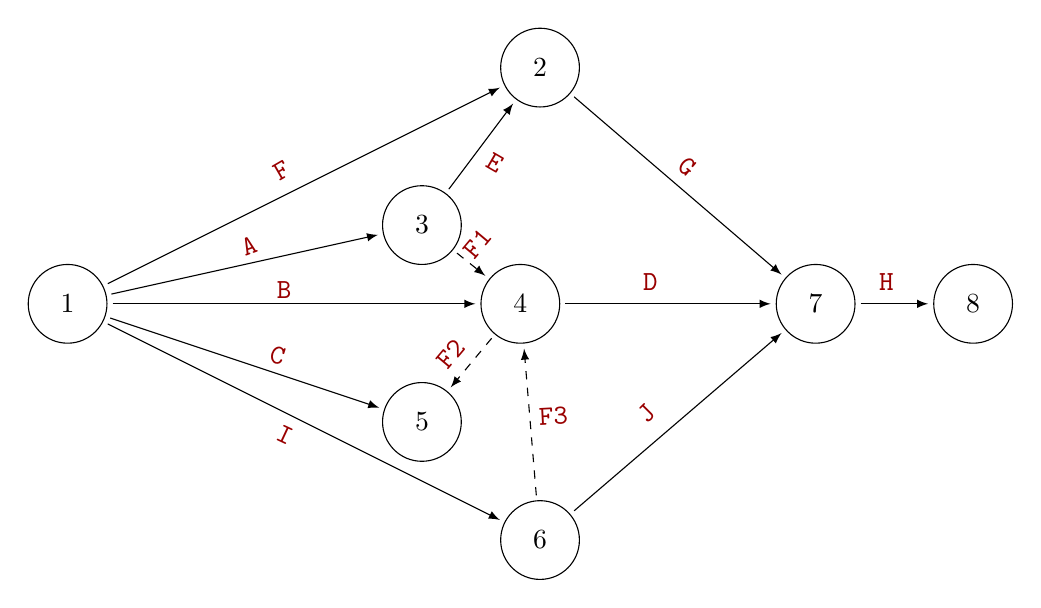
\begin{tikzpicture}[->, >=latex, node distance=2cm, every node/.style={draw, circle, minimum size=10mm, outer sep=2pt}]
		% Nodos
		\node (1) at (-2,0) {1};
		\node (2) at (4,3) {2};
		\node (3) at (2.5,1) {3};
		\node (4) at (3.75,0) {4}; %! modificado
		\node (5) at (2.5,-1.5) {5};
		\node (6) at (4,-3) {6};
		\node (7) at (7.5,0) {7};
		\node (8) at (9.5,0) {8};

		% Arcos
		\draw (1) -> (2);
		\draw (1) -> (6);
		\draw (1) -> (3);
		\draw (1) -> (5);
		\draw (1) -> (4);
		\draw (2) -> (7);
		\draw (4) -> (7);
		\draw[dashed] (3) -> (4);
		\draw (3) -> (2);
		\draw[dashed] (4) -> (5);
		\draw[dashed] (6) -> (4);
		\draw (6) -> (7);
		
		\draw (7) -> (8);
		%\draw (5) -> (7);
		%\draw[dashed] (1) -> (2);
		%\draw[bend left] (1) to (2);
		%\draw[dotted] (1) -> (2);
		%draw[bend right=45] (1) to (2);
		\path (1,1.2) node[draw=none, fill=none, rotate=30, above ,text=red!60!black] {\texttt{F}}; %* 1-2
		\path (0.5,0.2) node [draw=none, fill=none, rotate=20, above ,text=red!60!black] {\texttt{A}}; %* 1-3
		\path (0.75,-0.4) node [draw=none, fill=none, above ,text=red!60!black] {\texttt{B}}; %* 1-4
		\path (0.5,-1.2) node [draw=none, fill=none, rotate=-17, above ,text=red!60!black] {\texttt{C}}; %* 1-5
		\path (3.64,0.4) node [draw=none, fill=none, rotate=50, above ,text=red!60!black] {\texttt{F1}}; %* 3-4
		\path (3.3,-1) node [draw=none, fill=none, rotate=50, above ,text=red!60!black] {\texttt{F2}}; %* 5-4
		\path (4.2,-2) node [draw=none, fill=none, rotate=3, above ,text=red!60!black] {\texttt{F3}}; %* 4-6
		\path (5.5,1.3) node [draw=none, fill=none, rotate=-40, above ,text=red!60!black] {\texttt{G}}; %* 2-7
		\path (5.4,-0.3) node [draw=none, fill=none,  above ,text=red!60!black] {\texttt{D}}; %* 4-7
		\path (8.4,-0.3) node [draw=none, fill=none,  above ,text=red!60!black] {\texttt{H}}; %*7-8
		\path (5.75,-1.8) node [draw=none, fill=none,  above, rotate=45 ,text=red!60!black] {\texttt{J}}; %* 7-8
		\path (1,-1.15) node [draw=none, fill=none,  below,rotate = -25 ,text=red!60!black] {\texttt{I}}; %* 7-8
		\path (3.14,1.3) node [draw=none, fill=none, rotate=-30, above ,text=red!60!black] {\texttt{E}}; %* 3-4
	\end{tikzpicture}
\end{center}
\end{raggedright}
\end{document}
